\documentclass{article}
\usepackage[T1]{fontenc}
\usepackage[polish]{babel}
\usepackage[utf8]{inputenc}
\usepackage{listings}
\usepackage{graphicx}

\title{Kryptografia 2023 Exercise 5 List 1}
\author{Jakub Patałuch}

\begin{document}
Cryptography 2023, Exercise 5 from List 1, Jakub Patałuch
\section{Problem}
For authentication based on secret key K, we may have the problem of leaking the key to third 
parties. There might be different ways of such leakage, e.g. via delays in communication.


To protect ourselves against such leakage, we use a very large key K say, 100MB key. Then
leaking it bit by bit would take years. But how to use a large key so that:

\begin{enumerate}
    \item the adversary has a negligible chance to impersonate if he knows the bits of K on a fraction
    of 50\% positions,
    \item computing the authentication token (sent from the prover to the verifier) is very easy and fast.
\end{enumerate}

\section{Solution}

\subsection{Random Walk}
Let's consider a random walk performed on an array $D$ of size $2^k$, where every bit
is generater uniformly at random. Given a current position $p_i$, and a parameter $m$
the next position will be decided by a hash function $H$, in the following way:

\[p_{i+1} = H(D[i] \cdots D[i+m])\]

and $H: \{0,1\}^{m} \rightarrow \{0,1,\cdots,2^k-1\}$

We know from the previous exercise that:

\begin{enumerate}
    \item if $m < k-1$ then it is impossible to have a cycle that is the size of the array
    \item if $m \ge k-1$ then the propability of such cycle is negligible
\end{enumerate}

\subsection{Schema}

We will use the idea of random walks for our solution. The array $D$ will contains
bits of our key and an authentication token will be the position withing this array.
Given a starting position $p$, $m$ and a new paremeter $n$ which describes the amount
of steps our algorithms takes within array $D$, the algorithms is as follows:

\begin{lstlisting}[escapeinside={(*}{*)}]
    def getNthPosition(p, n, m, Hash, D):
        (*$p_0 \leftarrow p$*)
        for (*$i \leftarrow 1,\cdots ,n$*)
            (*$p_i \leftarrow Hash(D[p_{i-1} : p_{i-1}+m])$*)
        return (*$p_n$*)
\end{lstlisting}

If the $p_i + m > |D|-1$ the missing bits are taken from the front of the array.


We can assume that the $n, m$ and $Hash$ are standarized and are known to all parties.
With that the full authetnication schema is as follow:

\begin{center}
    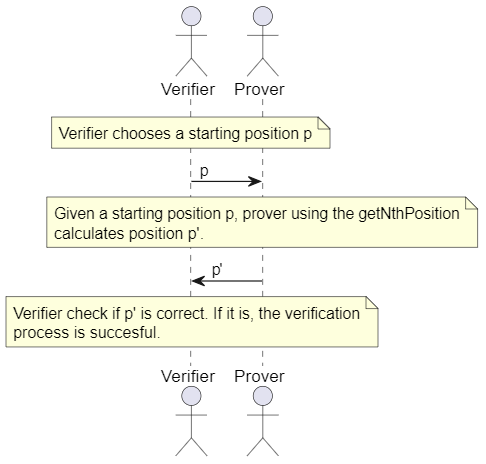
\includegraphics[
        width=10cm,
        keepaspectratio,
      ]{skima.png}
\end{center}

\subsection{Analysis}
\subsubsection{Impersonation chance for adversary}
Third party knows the algorithms, $n$, $m$, $Hash$, half of out key bits and the starting
position $p$. Having key the size of $100MB$ means that the $|D| \approx 8*10^8 \approx 2^{2.4*10^{8}}$

The safety of the schema depends heavly on the parameters that we choose. We will analyze few
possibilities.

\begin{itemize}
    \item $m = |D|$ 
\end{itemize}

When using full key, the adversary always knows precisly half of the input to hash function.
The probability of guessing the next step is: 
\[\frac{1}{2^{1.2*10^{8}}}\]
Even with only one step, the probability of adversary breaking our authentication is negligible.

\begin{itemize}
    \item $m <<< |D|$
\end{itemize}

Using entire key may be to expesive therefor we want to find smallest $m$ that still guarantees safety.
Let's temporary assume that the bits known by the attack are uniformly distributed and he always knows
half the hash function input. Probability of guessing the final position is
\[\frac{1}{2^{\frac{n*m}{2}}}\]
As long as $a*m \geq 512$ the schema is safe.

The problem arises when the bits known by attacker are grouped together. If the starting position and
every next position ends withing this group then the attack will succed. Assuming that $n << m$ and 
that hash function has a uniform distribution then probability of such situation is 
\[(\frac{1}{2^{a+1}})\]
See note A for more explanation.
This situation suggest, that large $n$ are needed. On example $n = 256$.

\section{Summary}
In summary this schema should be safe when both the $n$ and $m$ parameters are big. 
This however heavly impacts performance as hash function will be called hundreds of times.

A. As per $m$ having impact on the second attack scenario. $m$ is responsible for cycle lenght and
therefore final result should be 
\[\frac{1}{2^{min(a+1, cycle_lenght(p,m))}}\]

More analysis is requred but I runned out of time.
\end{document}